\section{Electron Dipole Moment, Path Integral for Gauge Fields}
Last lecture, we found the QED action:
\begin{equation}
    S = \int d^4x \bar{\psi}(i\slashed{\p} - m)\psi + A_\mu \bar{\psi}\gamma^\mu \psi + \frac{1}{4e^2}(F_{\mu\nu})^2 = \int d^4x\bar{\psi}(i\slashed{D} - m)\psi - \frac{1}{4e^2}F^2
\end{equation}
where in the second equality we introduce the covariant derivative:
\begin{equation}
    D_\mu \psi = \p_\mu \psi + iA_\mu \psi
\end{equation}
which is useful because it makes the action manifestly gauge invariant (you can observe that under a $U(1)$ transformation, the covariant derivative only picks up a phase).

\subsection{Magnetic dipole of the electron}
We do not yet know how to treat the gauge fields at a quantum-mechanical level. But even before going there, we can already make some predictions, just via treating the gauge fields classically. Namely, the electron is not just a point charge, but it also couples to the magnetic field, and we will see the prediction for its magnetic moment come out of the QED action.

\begin{center}
    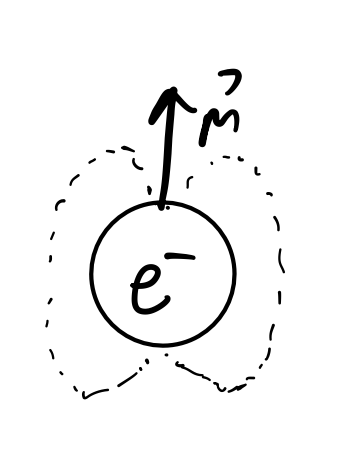
\includegraphics[scale=0.35]{Lectures/Images/lec8-emagmoment.png}
\end{center}

For a non-relativistic particle, we could consider a Zeeman coupling:
\begin{equation}
    H = \frac{(\v{p} + \v{A})^2}{2m} + \mu\v{B} \cdot \gv{\sigma}
\end{equation}
wherein the particle eigenstates $\ket{\v{p}, s = \pm}$ are based on the particle momenta $\v{p}$ and spin $s$. $\mu$ is the free parameter, which tells us the energy splitting between the two spin states (as a function of $B$):

\begin{center}
    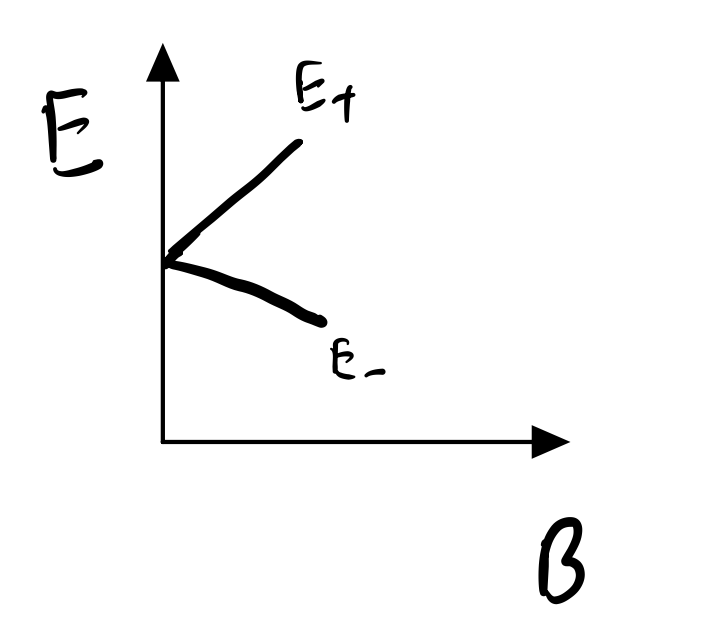
\includegraphics[scale=0.35]{Lectures/Images/lec8-energysplit.png}
\end{center}

Let's study the modified/gauged Dirac equation (the equation of motion in QED):
\begin{equation}
    0 = (i\slashed{D} + m)\psi
\end{equation}
and square it, in the way we derived Klein-Gordon equation from the regular dirac equation (This is how we derived the spectrum of free dirac fermions to be $E = \sqrt{p^2 + m^2}$):
\begin{equation}
    \begin{split}
        0 &= (i\slashed{D} + m)(-i\slashed{D} + m)\psi 
        \\ &= (\slashed{D}\slashed{D} + m^2)\psi
        \\ &= (\gamma^\mu\gamma^\nu D_\mu D_\nu + m^2)\psi
    \end{split}
\end{equation}
Now we write:
\begin{equation}
    \gamma^\mu\gamma^\nu = \frac{1}{2}\set{\gamma^\mu, \gamma^\nu} + \frac{1}{2}[\gamma^\mu, \gamma^\nu] = -\eta^{\mu\nu} - 2iS^{\mu\nu}
\end{equation}
with:
\begin{equation}
    S^{\mu\nu} = \frac{i}{4}[\gamma^\mu, \gamma^\nu]
\end{equation}
Thus:
\begin{equation}
    0 = (-D^2 - iS^{\mu\nu}2D_\mu D_\nu + m^2)\psi
\end{equation}
If we had no background ($A \to 0$), then the derivatives of $D_\mu D_\nu$ commute (hence symmetric), and its multiplied by an antisymmetric $S^{\mu\nu}$ and so the entire term vanishes. We are just left with the Klein-Gordon equation, as we expect. Since $2D_\mu D_\nu$ is contracted with $S^{\mu\nu}$, let us write it as:
\begin{equation}
    2D_{\mu}D_\nu \psi = (D_\mu D_\nu - D_\nu D_\mu)\psi
\end{equation}
where:
\begin{equation}
    D_\mu D_\nu \psi =  (\p_\mu + iA_\mu)(\p_\nu \psi + iA_\nu \psi) = \p_\mu \p_\nu \psi + i A_\nu \p_\mu \psi + i \p_\mu A_\nu \psi + i A_\mu \p_\nu \psi - A_\mu A_\nu \psi
\end{equation}
So the difference becomes (notice that most of the terms here are symmetric and cancel, with the exception of the $i\p_\mu A_\nu \psi$):
\begin{equation}
    [D_\mu, D_\nu]\psi = i(\p_\mu A_\nu - \p_\nu A_\mu)\psi = iF_{\mu\nu}\psi
\end{equation}
This is nice! Covariant derivatives are gauge invariant, and the thing we get out here is indeed a gauge invariant quantity.

Thus, returning to our equation of motion:
\begin{equation}
    0 = (-D^2 + S^{\mu\nu}F_{\mu\nu} + m^2)\psi
\end{equation}

Now, we want to study the energies of solutions to this equation when there is a magnetic field. We set $A_0 = 0$ and $\v{B} = \nabla \times \v{A}$. Only $F_{ij}$ are activated. What are the $S^{ij}$?:
\begin{equation}
    S^{ij} = \frac{i}{4}[\gamma^i, \gamma^j] = \frac{i}{4}\m{0 & \sigma^i \\ \bar{\sigma}^i & 0}\m{0 & \sigma^j \\ \bar{\sigma}^j & 0} - (i\leftrightarrow j) = \frac{i}{4}\m{[\sigma^i, \bar{\sigma}^j] & 0 \\ 0 & [\bar{\sigma}^i, \sigma^j]}
\end{equation}
Then looking at the relations that the Paulis satisfy:
\begin{equation}
    [\sigma^i, \sigma^j] = 2i\e^{ijk}\sigma_k
\end{equation}
we conclude:
\begin{equation}
    S^{ij} = \frac{1}{2}\e^{ijk}\m{\sigma^k & 0 \\ 0 & \sigma^k}
\end{equation}
Thus:
\begin{equation}
    S^{ij}F_{ij} = \frac{1}{2}\e^{ijk}\m{\sigma^k & 0 \\ 0 & \sigma^k} (\p_i A_j - \p_j A_i) = \m{\sigma^kB_k & 0 \\ 0 & \sigma^k B_k}
\end{equation}
So we have the full differential equation - to get the energies now all we need to do is fourier transform:
\begin{equation}
    E^2 = (\v{p} + \v{A})^2 + m^2 + \m{\gv{\sigma} \cdot \v{B} & 0 \\ 0 & \gv{\sigma} \cdot \v{B}}
\end{equation}
So the energy in the non-relativistic limit (wherein $m^2 \gg (\v{p} + \v{A})^2$) becomes:
\begin{equation}
    E = m\sqrt{1 + \frac{(\v{p} + \v{A})^2}{m^2} + \frac{1}{m^2} \m{\gv{\sigma} \cdot \v{B} & 0 \\ 0 & \gv{\sigma} \cdot \v{B}}} \approx m + \frac{(\v{p} + \v{A})^2}{2m} + \frac{1}{2m}\m{\gv{\sigma} \cdot \v{B} & 0 \\ 0 & \gv{\sigma} \cdot \v{B}}
\end{equation}
With the normalization of $A \to eA$ (the more familiar normalization from E\&M):
\begin{equation}
    E - m = \frac{(\v{p} + e\v{A})^2}{2m} + \frac{e}{2m}\gv{\sigma} \cdot \v{B}
\end{equation}
and thus:
\begin{equation}
    \boxed{\mu = \frac{e}{2m}}
\end{equation}
This is a nice and simple prediction, and one can compare it to experiments; we find:
\begin{equation}
    \mu = \frac{e}{2m}\cdot 1.0011597\ldots
\end{equation}
which is very close, but off! Why is it off? We treat the photon classically here, and there are quantum corrections. Pictorially, we can imagine that these corrections may look like (with the leftmost diagram the classical prediction):

\begin{center}
    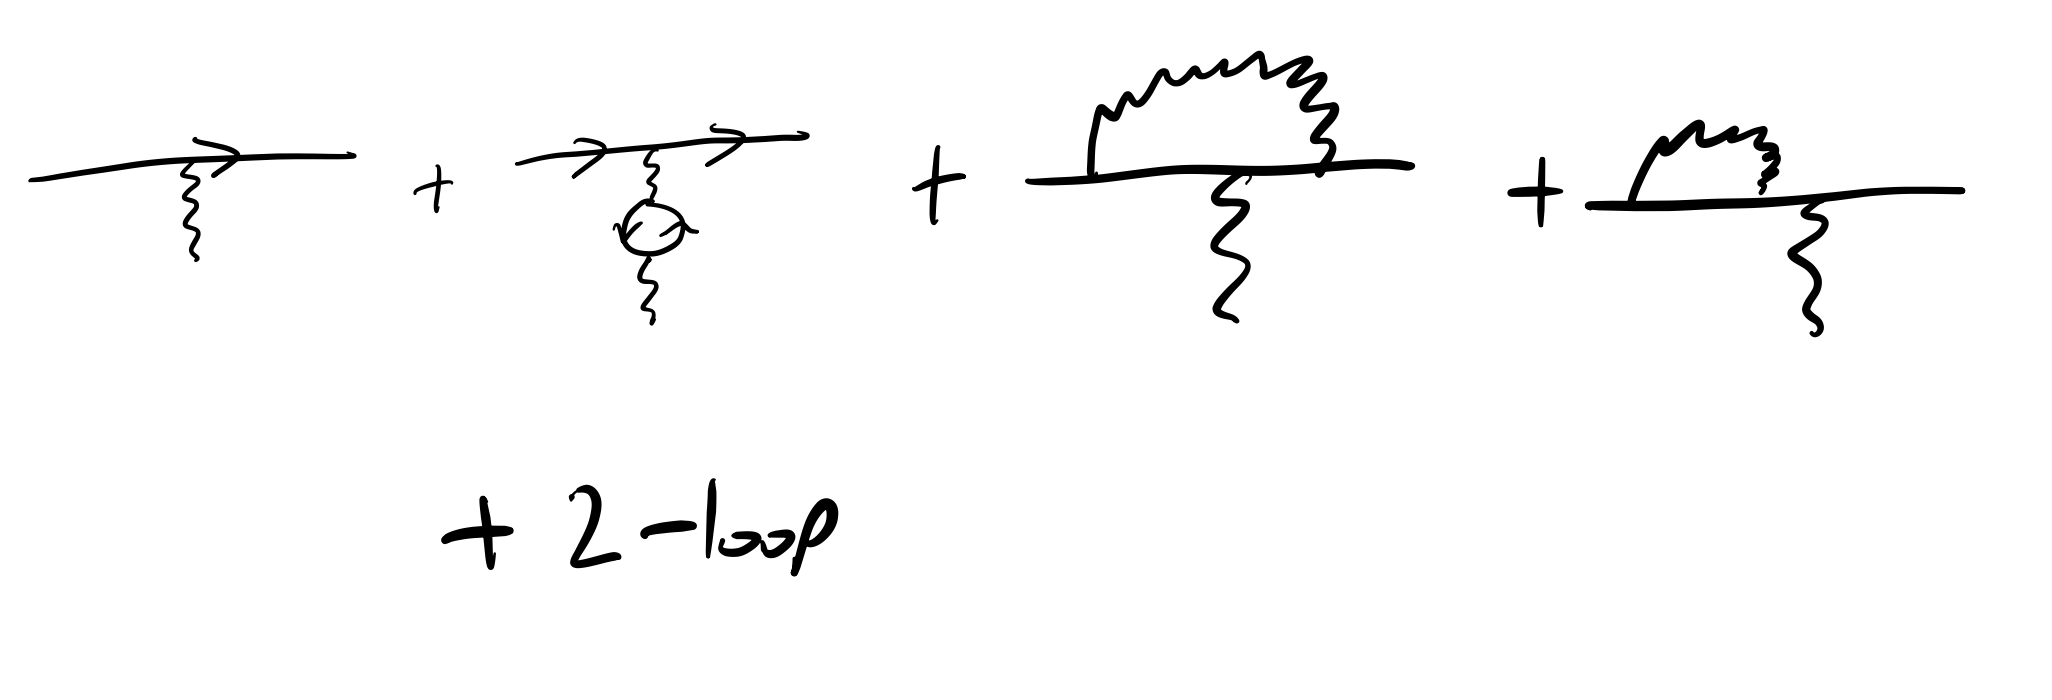
\includegraphics[scale=0.35]{Lectures/Images/lec8-mufeynmans.png}
\end{center}

The 1-loop corrections give the $0.00115$, and if you are braver and have a lot more time you can keep going, and the current agreement of theory and experiment is $10^{-13}$ (wow!) The dimensionless coupling in QED turns out to be small, which is why the perturbative expansion is useful here.

\subsection{Path Integral for Gauge Fields - First attempt}
Quantizing gauge fields is important not just for a more accurate prediction of the electron dipole, but in various aspects of particle and condensed matter physics. To do this, we jump straight to the path integral formulation. A good reference for this is Peskin 9.4, as well as Fradkin 9.5. We follow the approach by Fadeev and Popov approach. There are several advantages:
\begin{itemize}
    \item Path integrals! Much easier to calculate things
    \item Lorentz invariance is manifest
    \item Generalizes easily to quantization of non-abelian gauge fields
\end{itemize}
There are however alternatives you can read about, e.g. Gupta-Bleuler.

The naive guess for the path integral would be:
\begin{equation}
    Z = \int \mathcal{D}A_0 \mathcal{D}A_1 \mathcal{D}A_2 \mathcal{D}A_3 e^{iS_M[A]}
\end{equation}
with:
\begin{equation}
    S_M[A] = -\frac{1}{4}\int d^4x F^2
\end{equation}
and indeed this is not too far off. But it has some issues - namely due to gauge invariance. Loosely, gauge invariance tells us that there is a component of the gauge fields that does not enter into the action. So, one of the four integrals is over nothing. If this was it, it wouldn't be a huge problem, but there is a related larger problem; namely the kinetic term $\sim A\p\p A \sim AD A$ is not invertible (which is what we usually do to get the propagator). How do we see this? Well, looking at the Maxwell action:
\begin{equation}
    S_M[A] = -\frac{1}{4}\int_x F^2 = -\frac{1}{2}\int_x \p_\mu A_\nu (\p^\mu A^\nu - \p^\nu A_\mu) = \int_x A_\nu (\p^2 \eta^{\mu\nu} - \p^\nu \p^\mu)A_\mu
\end{equation}
and in momentum space this becomes:
\begin{equation}
    S_M[A] = -\int\frac{d^4p}{(2\pi)^4}A_\mu(-p)(p^2\eta^{\mu\nu} - p^\mu p^\nu) A_\nu(p)
\end{equation}
with $``D'' = (p^2\eta^{\mu\nu} - p^\mu p^\nu)$. Usually, we solve theories in the path integral formalism by coupling the theory to sources (say, $A_\mu J^\mu$) and complete the square to get something of the form $JD^{-1}J$. But here, $D$ is not invertible; indeed, we see this by acting $D$ on $p^\mu$:
\begin{equation}
    (p^2\eta^{\mu\nu} - p^\mu p^\nu)p^\mu = p^2p^\mu - p^2 p^\mu = 0
\end{equation}
i.e. $p^\mu$ is in the kernel of this matrix, and hence the matrix is not invertible. The underlying reason for this is due to the gauge invariance - ``Pure gauge configurations'' $A_\mu(x) = \p_\mu \lambda(x)$ have zero action and we should remove them/not be integrating over them.

A visual intuition; the space of gauge fields $A_\mu$ is large, but many of these fields are related via gauge transformations, and we integrate over these as well. The resolution is to choose a slice satisfying gauge fixing.

\begin{center}
    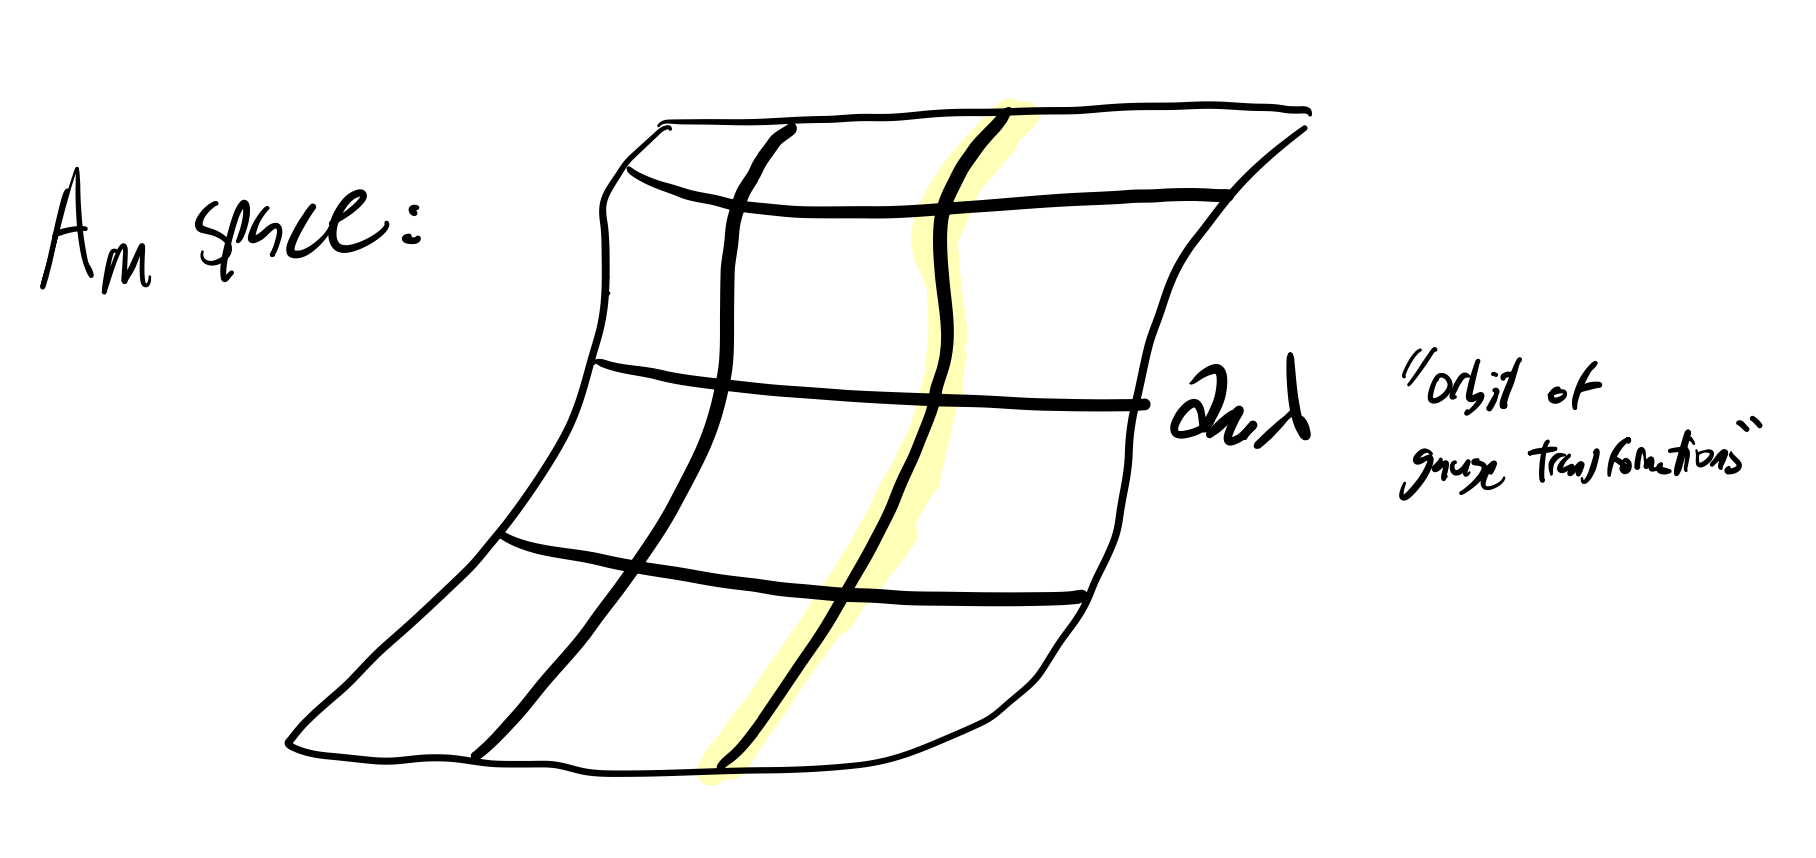
\includegraphics[scale=0.35]{Lectures/Images/lec8-gaugefields.png}
\end{center}

\subsection{Gauge Fixing in the Path Integral}
Consider a gauge-fixing condition:
\begin{equation}
    g(A_\mu) = \nabla \cdot \v{A} \;(\text{Coloumb}),\quad g(A_\mu) = \p_\mu A^\mu \;(\text{Lorenz}), \ldots
\end{equation}
After we fix a gauge, we can no longer relate different fields via gauge transformations, and we only integrate over ``true'' degrees of freedom. To this end would like to introduce something like $\delta(g(A))$ in the path integral. This will enforce that only configurations along a slice would enter the path integral.

To not mess things up, we will insert:
\begin{equation}
    1 = \int \mathcal{D}\lambda \delta(g(A_\lambda))\det \frac{\delta g(A_\lambda)}{\delta \lambda}
\end{equation}
where given $A_\mu$, $A^\lambda_\mu = A_\mu + \p_\mu \lambda$. The above expression is in analog to the single-variable function case, where $1 = \int dx \delta(f(x))\abs{f'(x)}$. So, our path integral then becomes:
\begin{equation}
    Z = \int \mathcal{D}\lambda \mathcal{D}A \delta(g(A^\lambda))\det \frac{\delta g(A_\lambda)}{\delta \lambda}e^{iS_M[A]}
\end{equation}
A comments; the path integral we started with is independent of any $g$, but since we insert 1, we don't introduce $g$ dependence (as should be the case, since we shouldn't expect fixing a gauge to change any of the physics). The introduction of this gauge fixing path integral will allow us to isolate the infinity/redundancy from the original path integral. Carrying on, note that the Maxwell equation is gauge invariant, so we can replace $A \to A_\lambda$. Therein only $A_\lambda$ appears in the integrand, so we can instead replace all variables with $A$, leaving the integrand $\lambda$-independent (note that the derivative term is also $\lambda$ independent, as we evaluate it at $A$ after taking the functional derivative):
\begin{equation}
    Z = \left(\int \mathcal{D}\lambda\right)\int \mathcal{D}A \delta(g(A))\left.\frac{\delta g(A^\lambda)}{\delta \lambda}\right|_A e^{iS_M[A]}
\end{equation}
Thus we have isolated the integral $\int \mathcal{D}\lambda$ over gauge orbits (that gives a factor of infinity) in a way that we can manifestly see it does nothing. Now we have an integral over $A$ with a delta function, which picks out a ``slice'' in gauge field space.

Now, this doesn't quite look like our regular Gaussian path integral, so we may have cause for worry. We will deal with this $\delta(g(A))$ by averaging over carefully chosen gauges. We consider:
\begin{equation}
    g_\omega(A) = \p_\mu A^\mu - \omega(x)
\end{equation}
the Lorenz gauge plus a function of spacetime. We average over these gauges with Gaussian weight:
\begin{equation}
    e^{i \int d^4x \frac{\omega^2(x)}{2\xi}}
\end{equation}
This trick will produce a Gaussian path integral!
\begin{equation}
    Z = \int \mathcal{D}A\mathcal{D}\omega e^{-i\int \frac{\omega^2(x)}{2\xi}}\delta(\p_\mu A^\mu - \omega)\det(\p^2)e^{-\frac{i}{4}\int_x F^2}
\end{equation}
An aside; the $\det(\p^2)$ term becomes much more interesting in the context of Non-Abelian gauge theories, as it then retains some dependence on $A$. Now, the $\omega$ integral is easy to evaluate, because we have a $\delta$ function fixing it:
\begin{equation}
    Z = \int \mathcal{D}Ae^{-i\int_x \frac{1}{4}F^2 + \frac{1}{2\xi}(\p_\mu A^\mu)^2}
\end{equation}
So what was the effect of all of this? We get an updated action:
\begin{equation}
    S = -\int d^4x \frac{1}{4}F^2 + \frac{1}{2\xi}(\p_\mu A^\mu)^2
\end{equation}
What's the point of doing this? Now, the kinetic term turns out to be invertible! Fourier transforming:
\begin{equation}
    S = -\int \frac{d^4p}{(2\pi)^4}A_\mu(-p)(\eta^{\mu\nu}p^2 - p^\mu p^\nu(1 - \frac{1}{\xi}))A_\nu(p)
\end{equation}
Let's find an inverse of:
\begin{equation}
    D^{\mu\nu} = \eta^{\mu\nu}p^2 - p^\mu p^\nu(1 - \frac{1}{\xi})
\end{equation}
via guessing; we want units of inverse $p^2$ and we want it to be Lorentz covariant with two indices, so our general guess is:
\begin{equation}
    (D^{-1})_{\mu\nu} = \frac{1}{p^2}(\eta_{\mu\nu} + \alpha\frac{p_\mu p_\nu}{p^2})
\end{equation}
Multiplying this out:
\begin{equation}
    (D^{-1})^{\mu\nu}D_{\nu\lambda} = (\eta^{\mu\nu} + \alpha\frac{p^{\mu}p^\nu}{p^2})(\eta_{\nu\lambda} - \frac{p_\nu p_\lambda}{p^2}(1 - \frac{1}{xi})) = \delta^{\mu}_\lambda \left(\alpha - \left(1 - \frac{1}{\xi}\right)\right)\frac{p^\mu p_\lambda}{p^2} - \alpha(1 - \frac{1}{\xi})\frac{p^\mu p_\lambda}{p^2}
\end{equation}
and we want the last terms to cancel which yields $\alpha = \xi - 1$. This gives a propagator we can invert, we can get the two-point function of the photon from this, and so on. We shall continue the discussion next week.